\textbf{COLUNI 2021 -- Questão 24}\par\medskip A Figura abaixo ilustra um experimento realizado em um laboratório de Ciências. Nele, a face inferior de uma barra metálica cilíndrica é colocada em um forno mantido a 70 °C. Depois de várias horas nessa condição, colocou-se um cubo de gelo com massa de 10 g sobre a extremidade superior da barra e mediu-se o tempo necessário para fundir completamente o gelo. Em seguida, realizou-se um novo experimento, idêntico ao anterior, exceto pelo fato de que a barra metálica foi substituída por outra. Observou-se que, no segundo experimento, o tempo necessário para fundir todo o gelo foi duas vezes maior.

\par

% COLUNI-AUTO-FIGURES-BEGIN
\begin{figure}[htbp]
\centering
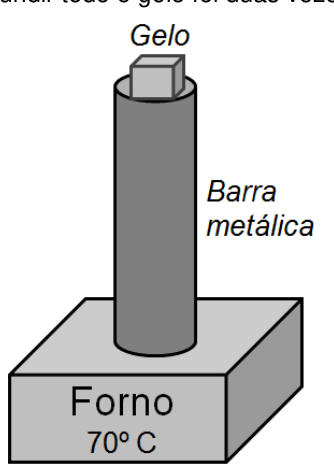
\includegraphics[width=0.95\linewidth]{static/simulados/coluni/figuras/2021/questao-24/figura-1.png}
\end{figure}
% COLUNI-AUTO-FIGURES-END

Considere as duas hipóteses abaixo sobre as barras utilizadas nos experimentos.

\par

I. É possível que as barras sejam constituídas do mesmo material e que a segunda tenha um comprimento menor e um diâmetro maior que aqueles da primeira barra. \\ 
II. É possível que as barras sejam constituídas de materiais diferentes e que tenham o mesmo comprimento e diâmetro.

\par

Com relação às afirmativas I e II, é CORRETO dizer que:

\begin{enumerate}
\item as duas afirmativas estão corretas.
\item nenhuma das afirmativas está correta.
\item apenas a afirmativa I está correta.
\item apenas a afirmativa II está correta.\end{enumerate}
